% !TeX root = chapter_01_why_risk_management_matters.tex
% Standalone Chapter 1 draft generated from Chapter_01_Why_Risk_Management_Matters.md.
\documentclass[11pt,openany]{book}
\usepackage{graphicx}
\usepackage{amsmath,amssymb}
\makeatletter
\def\input@path{{second_ed/style/}{../style/}}
\makeatother
\usepackage{erm_textbook_style}
\graphicspath{{second_ed/rscripts/chapter1/jnj_tylenol/}{../rscripts/chapter1/jnj_tylenol/}}
\providecommand{\tightlist}{\setlength{\itemsep}{0pt}\setlength{\parskip}{0pt}}
\emergencystretch=2em

\begin{document}

\chapter{Why Risk Management Matters}
\label{chap:why-risk-management-matters}

\begin{learningobjectives}
  \item Explain why corporate risk management appears irrelevant under perfect-market assumptions.
  \item Identify the assumptions behind the Modigliani--Miller propositions and the Capital Asset Pricing Model.
  \item Evaluate how taxes, distress costs, agency problems, information asymmetry, and regulation can make risk management valuable.
  \item Define the cost of risk and explain why minimizing it is not the same as eliminating risk.
  \item Apply the chapter's logic to a corporate crisis in which reputation, safety, and financial value interact.
\end{learningobjectives}

\chapteroverview{
This chapter addresses a fundamental puzzle in corporate finance: if shareholders can diversify away firm-specific risks in well-functioning capital markets, why should companies invest resources in risk management? We begin with the theoretical benchmark established by Modigliani and Miller (MM) and the Capital Asset Pricing Model (CAPM), which demonstrates that under idealized assumptions, corporate risk management decisions---such as hedging, insurance, and loss control---are irrelevant to firm value. We provide a detailed exposition of the assumptions underlying these irrelevance propositions and explain what they imply for corporate decision-making.

The second half of the chapter reverses this perspective, showing how violations of these idealized assumptions in the real world create opportunities for risk management to add value. Taxes, bankruptcy costs, agency problems, information asymmetries, investment constraints, and regulatory frictions all make corporate risk management potentially valuable. We introduce the concept of the \emph{cost of risk}---the total economic burden a firm bears because of uncertainty---and position risk management as a strategic tool to minimize this cost. By doing so, effective risk management frees resources for productive investment and growth. This chapter lays the conceptual foundation for the rest of the book, where we explore how to identify, measure, finance, and govern risks in practice.
}

\begin{corporateexample}[Johnson \& Johnson and the Tylenol Recall]
On the morning of \textbf{September 29, 1982}, a 12-year-old girl outside Chicago woke up with a cold. Her parents did what millions of American families did every week: they reached for a familiar red-and-white bottle of Extra-Strength Tylenol\index{Johnson and Johnson!Tylenol recall}\index{Tylenol recall}. She swallowed a capsule before school. Within hours, she was in critical condition. By the end of the day, she was dead.

At first, no one thought to blame the medicine. In the Chicago area that same day, a young postal worker came home complaining of pain, took Tylenol from the family bottle, and collapsed. His brother and sister-in-law rushed to his house to grieve---and each took a Tylenol for stress and headache from the same bottle. Both of them died as well. Another woman in a nearby suburb, and a woman recovering from childbirth, died after taking what they believed was the same pain reliever that millions of Americans trusted.

By \textbf{September 30}, police and doctors began to see a pattern. All of the victims had taken Extra-Strength Tylenol capsules shortly before they died. Tests on the remaining capsules in some of the bottles revealed something horrifying: they contained enough potassium cyanide to kill thousands of people. Someone had apparently taken Tylenol bottles off store shelves, opened them, replaced some of the capsules with poison, and quietly put the bottles back.

Tylenol was not a niche product. It was the leading over-the-counter pain reliever in the United States, with roughly a third of the market and an estimated \textbf{35 percent} share just before the murders. For Johnson \& Johnson, Tylenol generated hundreds of millions of dollars in annual sales and close to a fifth of corporate profits. Overnight, that success became the center of a national scare story.

In late September and early \textbf{October 1982}, television news carried nearly continuous coverage of the deaths, the investigation, and the possibility that more contaminated bottles might be in stores or homes. Police cruisers rolled slowly through neighborhoods with loudspeakers, warning residents not to take Tylenol. Pharmacies and supermarkets pulled Tylenol products from the shelves or taped handwritten warning signs on empty spaces. Hotlines lit up with calls from anxious consumers.

Inside Johnson \& Johnson's headquarters in New Jersey, the pressure was immense. No one yet knew how many bottles had been poisoned or where those bottles might be. There was no guarantee that the tampering was limited to the Chicago area. The company's leaders had to decide how far to go, and how fast, when every option was costly and the facts were incomplete.

On \textbf{October 5, 1982}, less than a week after the first death, Johnson \& Johnson ordered a \textbf{nationwide recall}\index{product recall} of Tylenol products: about \textbf{31 million bottles} with a retail value of more than \textbf{\$100 million} in 1982 dollars. At the same time, it halted Tylenol advertising, issued public warnings, set up toll-free numbers for consumers and hospitals, and cooperated closely with the Food and Drug Administration, the FBI, and local police.

From a narrow financial standpoint, this looked like a disaster. Tylenol's market share plunged about 20 percent within weeks, and corporate earnings were hit. Figure~\ref{fig:jnj-tylenol} shows Johnson \& Johnson's stock price over this period, normalized and plotted alongside the S\&P 500 index. Immediately after the \textbf{September 29} murders, the Johnson \& Johnson line drops sharply below the market index, indicating a substantial loss of market value relative to a diversified portfolio. In the weeks that follow, however, the line begins to recover. By \textbf{December 1982}, roughly two months after the initial recall, the Johnson \& Johnson price index has climbed back to approximately its pre-crisis level relative to the S\&P 500. The picture is a compact summary: the crisis and recall were costly in market value terms, but the company's actions---recall, communication, and redesign---helped restore investor confidence within a surprisingly short period.





Johnson \& Johnson did not stop with the recall. In \textbf{November 1982}, it reintroduced Tylenol capsules in new, triple-sealed, tamper-resistant packaging\index{tamper-resistant packaging}---foil seals, plastic neck bands, and other barriers that made it obvious if someone had opened the bottle. The company ran educational campaigns to explain the changes and offered discounts to bring customers back. Within a few years, Tylenol had regained its position as the top over-the-counter pain reliever in the country.

The Chicago Tylenol murders remain unsolved; no one has ever been convicted of the poisonings. Yet the episode is still cited as a clear example of a firm confronting a sudden, life-or-death problem and choosing to act quickly, openly, and at great cost to protect people and rebuild trust. It illustrates what is at stake in risk management: not only financial results, but also safety, reputation\index{reputation risk}, and the long-term viability of the enterprise.
\end{corporateexample}

\begin{figure}[htbp]
  \centering
  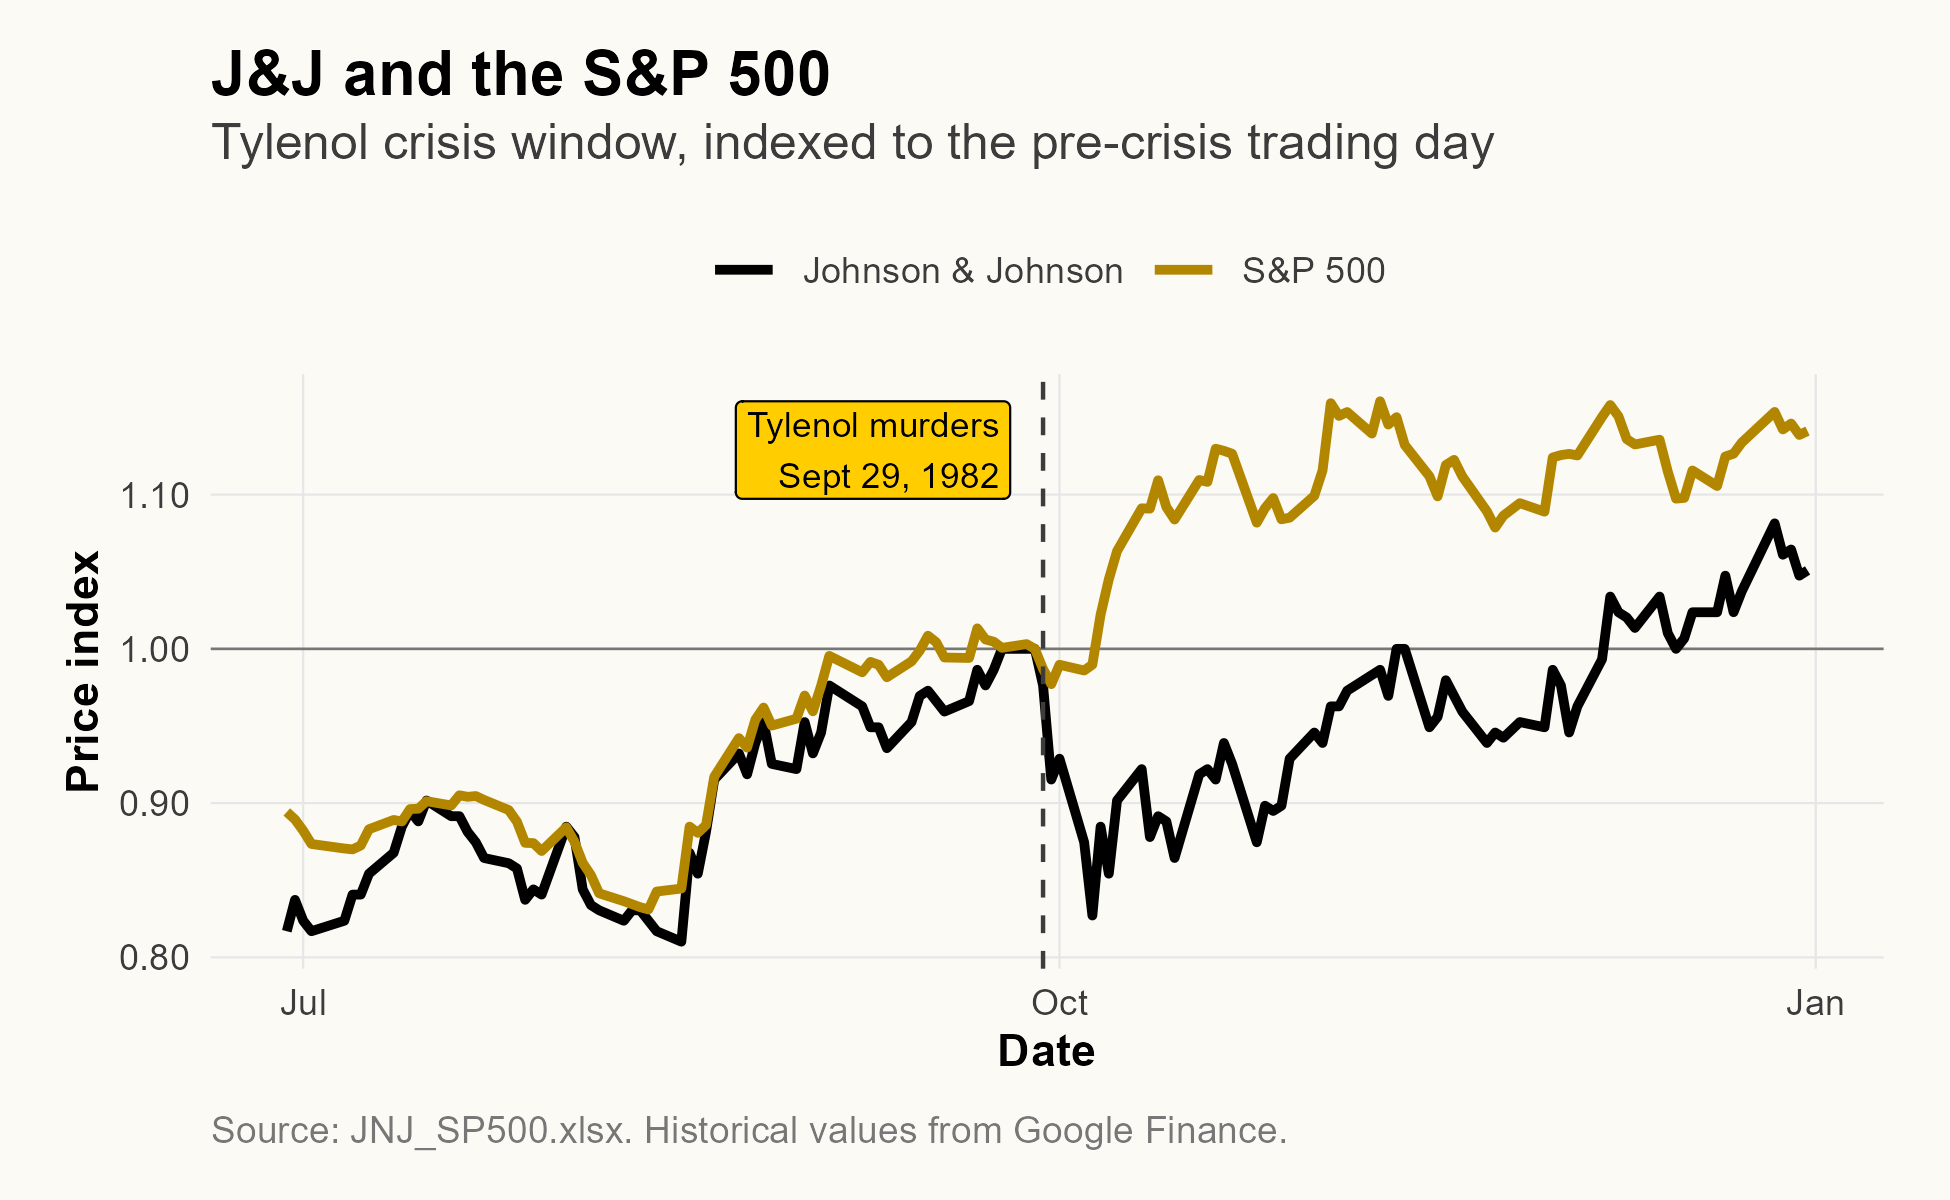
\includegraphics[width=\textwidth]{c1_jnjplot.png}
  \caption{Johnson \& Johnson's stock price fell sharply after the Tylenol murders, but the recovery by late 1982 suggests that the recall, communication strategy, and packaging redesign helped restore investor confidence.}
  \label{fig:jnj-tylenol}
  \figurenote{Both series are indexed to the last available trading day before September 29, 1982.}
\end{figure}

\section{Introduction: The Paradox of Risk Management}\label{introduction-the-paradox-of-risk-management}

Corporate risk management is a large and growing business. Firms purchase billions of dollars of insurance annually, employ sophisticated hedging strategies using derivatives, hire Chief Risk Officers\index{Chief Risk Officer (CRO)}, and establish elaborate risk management committees\index{risk committee} at the board level. Yet modern finance theory, rooted in the seminal work of Modigliani and Miller and the Capital Asset Pricing Model, suggests that under certain idealized conditions, these activities should be irrelevant to firm value. If capital markets are frictionless and investors can costlessly diversify away firm-specific risks, why should a corporation expend resources managing risks that shareholders can eliminate on their own?

This is the \emph{paradox of risk management}\index{risk management!paradox of}. In theory, risk management should not matter; in practice, it clearly does. Resolving this paradox is central to understanding enterprise risk management (ERM)\index{enterprise risk management (ERM)} and its role in corporate strategy.

The answer lies in recognizing that the assumptions underlying the irrelevance propositions---perfect capital markets, no taxes, no bankruptcy costs, symmetric information, and so on---do not hold in the real world. Each departure from these assumptions represents a \emph{friction}\index{market frictions} that can make risk management value-creating. Corporate risk management matters precisely because the idealized world of MM and CAPM does not exist. By reducing the impact of these frictions, risk management can increase firm value, lower the cost of capital, preserve financial flexibility, and improve decision-making.

This chapter proceeds in two parts. First, we carefully lay out the benchmark case: the assumptions and logic that lead to the irrelevance of risk management. Understanding this benchmark is essential; it tells us \emph{when} and \emph{why} risk management should not add value, and it provides a clear framework for identifying when it can. Second, we systematically examine the real-world frictions that break irrelevance and explain how risk management addresses each one. We conclude by introducing the \emph{cost of risk}\index{cost of risk}---a unifying concept that captures the total economic burden of uncertainty---and positioning the objective of corporate risk management as minimizing this cost subject to strategic goals.


\section{The Benchmark: Risk Management Is Irrelevant in Perfect Markets}\label{the-benchmark-risk-management-is-irrelevant-in-perfect-markets}

\subsection{The Modigliani--Miller Propositions}\label{the-modiglianimiller-propositions}

The Modigliani--Miller (MM) theorems\index{Modigliani-Miller propositions} are among the most influential results in corporate finance. In their 1958 paper, Modigliani and Miller demonstrated that, under a set of idealized assumptions, the value of a firm is independent of its capital structure. Whether a firm finances itself with debt or equity does not affect the total value available to all security holders. This result is sometimes called \emph{capital structure irrelevance}\index{capital structure irrelevance}.

The intuition is straightforward. In a perfect market, investors can replicate any capital structure on their own by borrowing or lending at the risk-free rate. If a firm is ``too conservative'' and holds little debt, an investor who prefers leverage can borrow personally to increase exposure. Conversely, if a firm is highly levered, an investor seeking less risk can lend at the risk-free rate to offset the firm's leverage. Because investors can costlessly undo the firm's financing decisions, those decisions do not affect firm value. The value of the firm is determined solely by its real assets and investment opportunities, not by how those assets are financed.

In subsequent work, Modigliani and Miller extended their analysis to dividend policy, again concluding irrelevance under the same frictionless assumptions. The logic generalizes to other corporate financial decisions, including risk management. If hedging, insurance, or other risk management activities merely rearrange cash flows without changing their expected present value, and if investors can replicate or undo these arrangements at zero cost, then risk management is irrelevant to firm value.

\subsection{The Capital Asset Pricing Model (CAPM)}\label{the-capital-asset-pricing-model-capm}

The Capital Asset Pricing Model\index{Capital Asset Pricing Model (CAPM)}, developed independently by Sharpe, Lintner, and others in the mid-1960s, provides a complementary perspective. CAPM describes the relationship between risk and expected return in equilibrium. According to CAPM, the expected return on any risky asset \emph{i} is:

\[
E[R_i] = R_f + \beta_i \left( E[R_M] - R_f \right)
\]

where:

\begin{itemize}
\tightlist
\item
  \(E[R_i]\) is the expected return on asset \emph{i},
\item
  \(R_f\) is the risk-free rate,
\item
  \(\beta_i\) measures the asset's sensitivity to the market portfolio,
\item
  \(E[R_M]\) is the expected return on the market portfolio.
\end{itemize}

The key insight of CAPM is that only \emph{systematic risk}\index{systematic risk}---risk that cannot be diversified away---is priced in equilibrium. Systematic risk, captured by beta\index{beta}, reflects the asset's covariance with the overall market. \emph{Idiosyncratic} or \emph{firm-specific} risk\index{idiosyncratic risk}, by contrast, can be eliminated by holding a diversified portfolio\index{diversification}. Because investors are assumed to hold well-diversified portfolios, they do not require compensation for bearing idiosyncratic risk.

For corporate risk management, the implication is stark: activities that reduce only firm-specific risk---such as insuring against fire, hedging commodity price exposure specific to one firm, or implementing loss control measures against operational hazards---do not reduce systematic risk and therefore do not lower the firm's cost of capital or increase its value. Investors can achieve the same risk reduction by diversifying their portfolios across many firms.

\subsection{Risk Management Irrelevance Under Perfect Markets}\label{risk-management-irrelevance-under-perfect-markets}

Combining the MM and CAPM logic, we arrive at the \emph{irrelevance of corporate risk management}\index{risk management!irrelevance of} under idealized conditions. If:

\begin{itemize}
\tightlist
\item
  Capital markets are perfect and frictionless,\index{perfect markets}
\item
  Investors can diversify away firm-specific risk costlessly,
\item
  There are no taxes, bankruptcy costs, or other distortions,
\end{itemize}

then corporate risk management decisions---hedging\index{hedging}, insurance, loss control spending---do not change firm value. Shareholders can replicate any risk profile they desire by adjusting their own portfolios. A firm that hedges its currency exposure, for example, merely substitutes stable cash flows for volatile ones without changing the expected present value of those cash flows. An investor who prefers the original, unhedged volatility can take offsetting positions in currency markets. Because risk management is redundant, it is irrelevant.

This benchmark does not mean risk management is useless or irrational. Rather, it establishes the conditions under which risk management would \emph{not} add value. It tells us that the rationale for corporate risk management must lie in violations of the perfect-market assumptions. Each friction or imperfection is a potential source of value creation through risk management.


\section{Assumptions Behind CAPM and MM Irrelevance}\label{assumptions-behind-capm-and-mm-irrelevance}

To understand when and why risk management matters, we must clearly articulate the assumptions underlying the irrelevance propositions. These assumptions define the idealized world in which risk management is redundant. In the following subsections, we list and explain these assumptions in detail.

\subsection{Detailed CAPM Assumptions}\label{detailed-capm-assumptions}

The Capital Asset Pricing Model rests on a set of strong assumptions\index{perfect markets!assumptions} about investor behavior and market structure. These assumptions are deliberately simplified to yield tractable predictions; they are not meant to be realistic descriptions of actual markets. Understanding them helps us identify where real-world departures create opportunities for value-adding risk management.

\textbf{Assumption 1: Frictionless Markets}

Markets are assumed to operate without transaction costs\index{transaction costs}, bid--ask spreads, or taxes. Investors can buy and sell any security instantly and costlessly. Securities are perfectly divisible, so investors can hold any fractional amount. There are no regulatory constraints, trading limits, or short-sale restrictions.

In such a world, adjusting one's portfolio is trivial. An investor can instantaneously and costlessly replicate or undo any risk management action a firm takes. This frictionless trading is essential to the irrelevance result: if trading were costly, investors might prefer firms to manage certain risks on their behalf.

\textbf{Assumption 2: Homogeneous Expectations}

All investors share identical beliefs about the expected returns, variances, and covariances of all assets. There is no disagreement about the probability distribution of future outcomes. Everyone uses the same information set and interprets it identically.

Homogeneous expectations ensure that all investors face the same investment opportunity set and agree on the efficient frontier. Without this assumption, different investors might value the same asset differently, and corporate risk management could serve to resolve or exploit these differences.

\textbf{Assumption 3: Single-Period Horizon}

All investors plan over a single, common time horizon. They care only about the distribution of wealth at the end of that period. There are no intermediate consumption needs, no differences in investment horizons, and no multi-period dynamic considerations.

This assumption simplifies the analysis by eliminating intertemporal concerns. In reality, firms and investors face multiple periods, varying liquidity needs, and evolving risks, which can make risk management valuable for managing cash flow timing and ensuring continuous access to capital.

\textbf{Assumption 4: Mean--Variance Preferences}

Investors care only about the mean and variance of portfolio returns.\index{mean-variance preferences} Higher expected return is desirable; higher variance is undesirable. Risk aversion is captured entirely by preferences over these two moments.

This assumption implies that investors are indifferent to higher moments (skewness, kurtosis) and that all risk is adequately summarized by variance. In practice, investors may care about downside risk, extreme events, and the shape of return distributions---concerns that motivate risk management tools like insurance and tail-risk hedging.

\textbf{Assumption 5: Risk-Free Asset and Unlimited Borrowing/Lending}

There exists a risk-free asset offering a known, certain return. All investors can borrow or lend unlimited amounts at this risk-free rate without constraints or credit limits.

In reality, borrowing rates typically exceed lending rates, and borrowing capacity is limited, especially during crises. Firms and investors face collateral constraints and varying access to credit. These imperfections can make internal cash flow stability---enhanced by risk management---valuable for maintaining investment.

\textbf{Assumption 6: All Assets Are Tradable and Marketable}

Every source of risk can be bought, sold, and held in a diversified portfolio. There are no non-traded risks such as private human capital, reputation, or firm-specific knowledge.

In practice, many important risks are not tradable. Managers' human capital is firm-specific and cannot be diversified. Reputation and customer relationships are intangible and illiquid. These non-traded risks can make managers more risk-averse than diversified shareholders, creating a role for corporate risk management to align interests.

\textbf{Assumption 7: Perfect and Symmetric Information}

All information relevant to asset valuation is costlessly and instantly available to all investors. There is no information asymmetry between managers and shareholders, or among investors. Everyone observes the same signals and interprets them identically.

In reality, managers typically know more about their firm's risks and prospects than outside investors do. This information asymmetry can lead to adverse selection and moral hazard\index{moral hazard} problems. Risk management and disclosure policies can mitigate these problems, improving firm value.

\textbf{Assumption 8: No Bankruptcy or Financial Distress Costs}

Default and financial distress are costless events. Bankruptcy is simply a transfer of ownership from equity holders to debt holders, with no loss of value in the process. There are no legal fees, no lost customers, no disrupted operations.

In practice, bankruptcy and financial distress impose substantial direct costs (legal and administrative expenses) and indirect costs (lost customers, suppliers demanding stricter terms, key employees departing). Risk management that reduces the probability of distress can therefore add value.

\textbf{Assumption 9: No Taxes or Neutral Tax Treatment}

There are no corporate or personal taxes, or taxes are neutral and symmetric (gains and losses treated identically, no progressivity, unlimited loss carryforwards and carrybacks at full value).

Real tax systems are not neutral. Corporate tax rates may be progressive, loss offsets are limited, and tax timing matters. Volatile income can increase expected taxes due to convexity and loss limitations. Risk management that smooths taxable income can reduce expected tax liabilities.

\textbf{Assumption 10: No Agency Costs or Conflicts of Interest}

Managers act perfectly in the interests of shareholders. There are no conflicts between managers and owners, or between different classes of security holders. Compensation contracts align incentives perfectly.

In reality, managers have their own objectives, which may not fully align with shareholder value maximization. Risk management and governance mechanisms help mitigate these agency problems and can increase firm value.

\subsection{Modigliani--Miller Assumptions (Overlapping with CAPM)}\label{modiglianimiller-assumptions-overlapping-with-capm}

The MM irrelevance propositions rely on similar assumptions:

\begin{enumerate}
\def\labelenumi{\arabic{enumi}.}
\tightlist
\item
  \textbf{No taxes} (or neutral, symmetric tax treatment).
\item
  \textbf{No transaction or issuance costs} for securities.
\item
  \textbf{Symmetric information} between managers and investors.
\item
  \textbf{No bankruptcy or financial distress costs.}
\item
  \textbf{Firms and individuals can borrow and lend at the same rates} (perfect capital markets).
\item
  \textbf{Investment policy is fixed and independent of financing decisions} (no underinvestment or overinvestment problems).
\end{enumerate}

The overlap between CAPM and MM assumptions is substantial. Both models rely on frictionless markets, perfect information, no taxes, and no distress costs. The irrelevance of risk management follows naturally: if shareholders can costlessly replicate or undo the firm's risk management actions, those actions do not affect firm value. The firm's value depends only on its real investment opportunities and the systematic risk of its cash flows.

\subsection{What Irrelevance Means}\label{what-irrelevance-means}

Understanding irrelevance is crucial. Irrelevance does \emph{not} mean that risk or risk management is unimportant in some absolute sense. Rather, it means that, under the stated assumptions, corporate risk management decisions do not affect firm value because they are redundant. Anything the firm does to manage risk can be undone or replicated by shareholders in their own portfolios at zero cost.

For example:

\begin{itemize}
\tightlist
\item
  If a firm hedges interest rate exposure, a shareholder who wants that exposure can take an offsetting position in interest rate derivatives.
\item
  If a firm buys fire insurance, a diversified shareholder already holds a portfolio that averages away the idiosyncratic fire risk across many firms.
\item
  If a firm smooths earnings through hedging, investors can ``see through'' the smoothing and value the firm based on its underlying cash flows.
\end{itemize}

Irrelevance is a powerful benchmark because it isolates the question: \emph{What conditions must fail for risk management to add value?} The answer is that real-world frictions---taxes, distress costs, agency problems, information asymmetries, regulatory constraints, and investment inflexibilities---break irrelevance and create opportunities for value-enhancing risk management.


\section{Real-World Frictions That Make Risk Management Matter}\label{real-world-frictions-that-make-risk-management-matter}

The value of corporate risk management arises from violations of the perfect-market assumptions. Each friction represents a wedge between the idealized benchmark and actual corporate finance. In this section, we examine the major frictions and explain how risk management can mitigate their costs, thereby increasing firm value.

\subsection{Taxes and Tax Convexity}\label{taxes-and-tax-convexity}

\textbf{The Friction: Progressive and Convex Tax Schedules}

Real corporate tax systems are not neutral.\index{taxes!and risk management} Tax rates may be progressive, rising with income. Losses and gains are not treated symmetrically: losses can often be carried forward or back, but with limitations. Net operating loss carryforwards\index{net operating loss carryforwards} may expire, and their present value is reduced by discounting and uncertainty. In some jurisdictions, the tax code includes exemptions, deductions, and credits that phase in or out, creating convexity in the effective tax schedule\index{tax convexity}.

\textbf{How Volatility Increases Expected Taxes}

When the tax function is convex, Jensen's inequality\index{Jensen's inequality} implies that the expected tax liability on a volatile stream of income exceeds the tax liability on a stable stream with the same expected value. Intuitively, in high-income years the firm pays tax at a high marginal rate, while in low-income (or loss) years, the tax benefit of losses is limited or delayed. Averaging over many periods, the volatile firm pays more in expected present-value taxes than a stable firm with identical expected income.

\textbf{Simple Example}

Consider a firm facing a progressive tax schedule:

\begin{itemize}
\tightlist
\item
  Income below \$100 million: 20\% tax rate.
\item
  Income above \$100 million: 30\% tax rate.
\end{itemize}

Firm A (stable): Earns \$100 million each year. Tax: \$20 million per year.

Firm B (volatile): Earns \$50 million in bad years, \$150 million in good years (average \$100 million). In bad years: tax = \$10 million. In good years: tax on first \$100 million = \$20 million, tax on next \$50 million = \$15 million, total = \$35 million. Average tax = \(\frac{10 + 35}{2} = \$22.5\) million.

Firm B pays \$2.5 million more in expected taxes annually solely because of volatility, even though expected pre-tax income is the same.

\textbf{How Risk Management Adds Value}

By using hedging, insurance, or other tools to smooth taxable income, risk management reduces the expected present value of taxes. Reducing income volatility shifts the firm toward the stable case, lowering the average tax rate. The tax savings increase after-tax cash flows and firm value.

This friction is one of the most straightforward and empirically supported rationales for corporate hedging and risk management.

\subsection{Costly Financial Distress and Bankruptcy}\label{costly-financial-distress-and-bankruptcy}

\textbf{The Friction: Bankruptcy Is Not Costless}

Under the MM assumptions, bankruptcy is merely a transfer of ownership from equity holders to debt holders, with no destruction of value. In reality, bankruptcy and financial distress impose significant costs:\index{financial distress!costs of}\index{bankruptcy costs}

\begin{itemize}
\tightlist
\item
  \textbf{Direct costs}: Legal fees, court costs, advisory fees, and administrative expenses. These costs can consume a substantial fraction of firm value, especially for smaller firms.
\item
  \textbf{Indirect costs}: Before and during bankruptcy, customers may flee (fearing disrupted service or warranty claims), suppliers may demand stricter payment terms or refuse to deal, key employees may depart, and the firm may lose valuable intangible assets like reputation and brand. Investment and innovation often stall. Competitors may poach market share.
\end{itemize}

Studies suggest that direct costs alone can be 3--5\% of firm value, and indirect costs can be much larger, sometimes exceeding 10--20\% of pre-distress value for firms in industries where reputation and customer confidence are critical.

\textbf{How Volatility Increases Distress Costs}

High volatility of cash flows and earnings increases the probability that the firm will face financial distress or default, especially if the firm is leveraged. The expected cost of distress is:

\[
\text{Expected Distress Cost} = \Pr(\text{Distress}) \times \text{Cost if Distressed}
\]

By increasing \(\Pr(\text{Distress})\), volatility raises the expected distress cost, reducing firm value.

\textbf{How Risk Management Adds Value}

Risk management reduces cash flow volatility, which in turn reduces the probability of distress. For example:

\begin{itemize}
\tightlist
\item
  Hedging commodity price or currency risks stabilizes operating cash flows.
\item
  Purchasing insurance\index{insurance} against property damage, liability, or business interruption\index{business interruption} ensures that large, unexpected losses do not push the firm into distress.
\item
  Managing liquidity through credit lines or cash reserves provides a buffer against shocks.
\end{itemize}

By lowering the expected present value of distress costs, risk management increases firm value. This benefit is particularly large for highly leveraged firms or firms in industries with high indirect distress costs.

\subsection{Investment Distortions and Underinvestment}\label{investment-distortions-and-underinvestment}

\textbf{The Friction: Financial Constraints and Limited Access to External Capital}

The MM framework assumes that firms can always finance positive-NPV projects by issuing securities at fair prices. In reality, external finance is costly and often limited, especially during downturns or after negative shocks. Asymmetric information and agency problems raise the cost of external capital. During crises or firm-specific shocks, access to capital markets may dry up entirely, or new equity can be issued only at a steep discount.

\textbf{The Underinvestment Problem}

When a firm faces a valuable investment opportunity but lacks internal funds and cannot raise external capital at reasonable terms, it may forgo the project. This is the \emph{underinvestment problem}\index{underinvestment problem}, famously analyzed in the context of debt overhang\index{debt overhang} and financial constraints. Missing positive-NPV projects reduces firm value.

Volatile cash flows exacerbate underinvestment. If the firm's cash flows are highly uncertain, it is more likely to find itself short of funds precisely when investment opportunities arise. Without hedging or insurance, internal funds may be depleted by unrelated shocks (e.g., commodity price swings, currency losses, catastrophic property damage), forcing the firm to pass on valuable projects.

\textbf{How Risk Management Adds Value}

Risk management smooths and stabilizes internal cash flows. By doing so, it ensures that the firm has predictable funds available to seize investment opportunities as they arise. This is sometimes described as \emph{preserving financial flexibility}\index{financial flexibility} or \emph{protecting the option to invest}.

\textbf{Simple Example}

Consider a firm with a valuable growth project requiring \$50 million. The firm's internal cash flow is either \$30 million (bad state) or \$70 million (good state), each with 50\% probability. External finance is costly or unavailable.

\begin{itemize}
\tightlist
\item
  \textbf{Without hedging}: In the bad state, the firm cannot fund the project (shortfall of \$20 million). The firm loses the NPV of the project in that state. Expected loss = 50\% of project NPV.
\item
  \textbf{With hedging}: The firm smooths cash flow to \$50 million in each state (paying in good states, receiving in bad states). Now the firm can fund the project in \emph{all} states. Expected loss = 0.
\end{itemize}

By enabling consistent investment, risk management captures the full expected NPV of the project, increasing firm value.

This rationale is empirically important. Studies find that firms with greater cash flow volatility invest less, and that hedging is positively associated with investment, especially for financially constrained firms.

\subsection{Principal--Agent Problems and Managerial Incentives}\label{principalagent-problems-and-managerial-incentives}

\textbf{The Friction: Misaligned Incentives Between Managers and Shareholders}

MM and CAPM assume that managers act perfectly in shareholders' interests. In reality, managers are agents of shareholders (the principals), and their incentives are not perfectly aligned. This creates \emph{agency costs}\index{agency costs}\index{principal-agent problem}.

Managers face firm-specific risks that they cannot diversify away:

\begin{itemize}
\tightlist
\item
  Their human capital\index{human capital!managerial} is tied to the firm. If the firm performs poorly or fails, the manager loses income, reputation, and future career prospects.
\item
  Managerial compensation is often closely tied to firm performance (salary, bonus, equity grants).
\end{itemize}

As a result, managers may be more risk-averse than well-diversified shareholders, leading them to avoid risky (but positive-NPV) projects or to over-invest in hedging and insurance beyond what shareholders would prefer.

Conversely, under some compensation structures (e.g., heavy reliance on stock options), managers may become \emph{too} risk-loving, taking excessive risks to increase the option value of their compensation (``gambling for resurrection'')\index{gambling for resurrection}.

\textbf{How Risk Management Can Align Incentives}

Well-designed risk management and governance can help align managerial risk-taking with shareholder preferences:

\begin{enumerate}
\def\labelenumi{\arabic{enumi}.}
\item
  \textbf{Reducing uncompensated managerial risk aversion}: By hedging or insuring risks that are unrelated to the firm's core strategy (e.g., commodity price risk for a non-commodity firm), risk management reduces volatility that worries managers but does not concern diversified shareholders. This frees managers to take value-creating strategic risks.
\item
  \textbf{Constraining excessive risk-taking}: Board-level risk limits, hedging policies, and enterprise-wide risk frameworks can prevent managers from ``gambling'' with firm assets when compensation incentives are misaligned. Risk committees and independent oversight complement compensation design.
\item
  \textbf{Improving performance measurement and incentive contracting}: By smoothing noise and clarifying performance, risk management makes it easier to design effective incentive contracts. Cleaner signals of managerial effort and skill improve the efficiency of compensation.
\end{enumerate}

\textbf{Example}

A CEO whose wealth is heavily invested in company stock may be reluctant to undertake a risky (but high-NPV) international expansion because failure could devastate her personal wealth. If the firm hedges exchange rate and political risks associated with the expansion, the CEO's personal risk is reduced, and she is more willing to pursue the value-creating project. The hedging realigns her incentives with those of diversified shareholders.

\subsection{Information Asymmetry and Signaling}\label{information-asymmetry-and-signaling}

\textbf{The Friction: Managers Know More Than Investors}

Perfect markets assume symmetric information. In reality, managers possess private information about the firm's risks, opportunities, and prospects. This \emph{information asymmetry}\index{information asymmetry} creates several problems:

\begin{itemize}
\tightlist
\item
  \textbf{Adverse selection}\index{adverse selection}: Investors cannot perfectly distinguish high-quality firms from low-quality ones. They demand a risk premium to compensate for uncertainty, raising the firm's cost of capital.
\item
  \textbf{Undervaluation}: Good firms may be systematically undervalued if investors cannot observe quality. This can lead to underinvestment in equity or foregone opportunities.
\item
  \textbf{Earnings opacity}: Volatile, hard-to-interpret earnings make it difficult for investors to assess managerial performance and firm fundamentals, again increasing required returns.
\end{itemize}

\textbf{How Risk Management Reduces Information Asymmetry}

Risk management can improve the transparency and credibility of the firm's reported performance:

\begin{enumerate}
\def\labelenumi{\arabic{enumi}.}
\item
  \textbf{Smoothing idiosyncratic noise}: Hedging and insurance reduce volatility from sources unrelated to managerial actions or strategic choices. This makes it easier for investors to identify the firm's core performance and prospects. For example, hedging currency risk allows investors to evaluate operating performance without the noise of exchange rate fluctuations.
\item
  \textbf{Signaling quality}\index{signaling}: A firm's willingness to commit to risk management policies can serve as a credible signal. For example, a firm that hedges consistently may signal confidence in its core business and a long-term orientation, differentiating itself from opportunistic or lower-quality competitors.
\item
  \textbf{Reducing cost of capital}\index{cost of capital}: Lower information asymmetry reduces the adverse selection premium investors demand, lowering the firm's cost of equity and debt.
\end{enumerate}

\textbf{Example}

Consider two firms with identical expected operating income but different hedging policies. Firm A hedges its commodity exposure; Firm B does not. Firm B's reported earnings are volatile, partly due to commodity price swings. Investors cannot easily separate operational performance from commodity luck. They demand a higher return to compensate for this uncertainty. Firm A's hedged earnings are more stable and informative, reducing the information premium and lowering the cost of capital.

\subsection{Contracting and Stakeholder Relationships}\label{contracting-and-stakeholder-relationships}

\textbf{The Friction: Long-Term Relationships Are Sensitive to Firm Risk}

Firms operate within a web of relationships: employees, customers, suppliers, distributors, regulators, and communities.\index{stakeholder relationships} Many of these relationships involve explicit or implicit long-term contracts\index{implicit contracts}. For example:

\begin{itemize}
\tightlist
\item
  Employees expect stable employment and career development.
\item
  Customers rely on warranties, service, and product quality.
\item
  Suppliers invest in relationship-specific assets.
\item
  Distributors commit resources to promote the firm's products.
\end{itemize}

These relationships are vulnerable to firm distress. If a firm experiences a severe negative shock, it may:

\begin{itemize}
\tightlist
\item
  Lay off workers, breaking implicit employment commitments.
\item
  Cut quality or service, damaging customer trust.
\item
  Default on supplier payments, disrupting the supply chain.
\item
  Lose regulatory licenses or face stricter oversight.
\end{itemize}

\textbf{How Volatility Damages Relationships}

High volatility increases the risk of extreme negative outcomes that jeopardize relationships. Stakeholders---who are not diversified with respect to this specific firm---will demand compensation for bearing this risk or will reduce their commitment. For example:

\begin{itemize}
\tightlist
\item
  Employees may demand higher wages to compensate for job insecurity, or top talent may leave for more stable firms.
\item
  Customers may avoid products from a financially unstable firm (especially for durable goods or products requiring after-sale support).
\item
  Suppliers may demand cash-in-advance or refuse credit.
\item
  Lenders and bondholders will demand higher interest rates.
\end{itemize}

\textbf{How Risk Management Protects Relationships}

By reducing the probability of extreme adverse outcomes, risk management helps the firm honor implicit and explicit commitments:

\begin{itemize}
\tightlist
\item
  Insurance and hedging make it more likely the firm can maintain employment during downturns.
\item
  Product liability insurance and quality controls credibly commit the firm to stand behind its products, enhancing brand and sales.
\item
  Financial stability allows the firm to negotiate better terms with suppliers and distributors.
\end{itemize}

The result is lower contracting costs and more valuable long-term relationships, increasing firm value.

\subsection{Regulatory and Rating-Agency Constraints}\label{regulatory-and-rating-agency-constraints}

\textbf{The Friction: Capital Requirements, Regulation, and Credit Ratings}

Many industries are subject to regulatory oversight that ties capital requirements or operating permissions to measures of financial stability:

\begin{itemize}
\tightlist
\item
  \textbf{Banks and insurers} face risk-based capital requirements\index{capital requirements!regulatory}. Volatile earnings and capital ratios can trigger regulatory intervention or require costly capital raises.
\item
  \textbf{Utilities} are regulated and their rate-setting depends on perceived risk and cost of capital.
\item
  \textbf{Credit ratings}\index{credit ratings}: Rating agencies\index{rating agencies} penalize earnings volatility and reward consistent risk management. Higher ratings reduce borrowing costs and improve access to capital markets.
\end{itemize}

\textbf{How Risk Management Adds Value Under Regulation}

Risk management that reduces volatility and smooths capital ratios helps firms:

\begin{itemize}
\tightlist
\item
  Maintain or improve credit ratings, lowering the cost of debt and expanding the investor base.
\item
  Avoid breaching regulatory capital thresholds, which can trigger expensive corrective actions or restrict business growth.
\item
  Demonstrate prudent governance to regulators, reducing the risk of additional regulation or penalties.
\end{itemize}

\textbf{Example}

An insurance company that uses reinsurance\index{reinsurance} and hedging to reduce underwriting volatility will have more stable surplus levels. This stability supports a higher credit rating, which in turn allows the company to write more business at better terms and reduces its cost of debt. The value created by improved ratings and regulatory standing justifies the cost of reinsurance and hedging.


\section{The Cost of Risk and the Objective of Corporate Risk Management}\label{the-cost-of-risk-and-the-objective-of-corporate-risk-management}

\subsection{Defining the Cost of Risk}\label{defining-the-cost-of-risk}

After examining the frictions individually, it is useful to introduce a unifying framework: the \emph{cost of risk}\index{cost of risk!components}. The cost of risk is the total economic burden a firm bears because its future outcomes are uncertain. It includes both direct costs (such as insurance premiums and retained losses) and indirect costs (the value destroyed by volatility through taxes, distress, agency, information, and regulatory channels).

We can express the cost of risk schematically as:

\[
\begin{aligned}
\text{Cost of Risk} ={}& \text{Expected Retained Losses} + \text{Risk Control Costs} \\
&+ \text{Risk Financing Costs} + \text{Indirect Costs of Volatility}
\end{aligned}
\]

\textbf{Components:}

\begin{enumerate}
\def\labelenumi{\arabic{enumi}.}
\item
  \textbf{Expected Retained Losses}\index{retained losses}: The present value of losses the firm will bear directly (deductibles, uninsured losses, etc.).
\item
  \textbf{Risk Control Costs}\index{loss control}: Expenditures on loss prevention, safety programs, quality control, cybersecurity, and other measures to reduce the frequency or severity of losses.
\item
  \textbf{Risk Financing Costs}\index{risk financing}: Premiums for insurance, fees for hedging instruments, costs of maintaining credit lines, and administrative costs of risk management programs.
\item
  \textbf{Indirect Costs of Volatility}: The deadweight losses arising from frictions:

  \begin{itemize}
  \tightlist
  \item
    Increased expected taxes due to convexity.
  \item
    Expected bankruptcy and distress costs.
  \item
    Underinvestment and foregone positive-NPV projects.
  \item
    Agency costs and misaligned incentives.
  \item
    Information asymmetry and higher cost of capital.
  \item
    Damaged stakeholder relationships.
  \item
    Regulatory penalties or increased capital requirements.
  \end{itemize}
\end{enumerate}

\subsection{The Objective of Corporate Risk Management}\label{the-objective-of-corporate-risk-management}

The goal of corporate risk management is \emph{not} to eliminate all risk. Risk is inseparable from return; eliminating risk would also eliminate profitable opportunities. Rather, the objective is to \textbf{minimize the total cost of risk, subject to the firm's strategic goals and risk appetite}\index{cost of risk!minimization}\index{risk appetite}.

In practice, this means:

\begin{itemize}
\tightlist
\item
  Identifying and measuring the firm's key risks.
\item
  Deciding which risks to retain\index{risk retention} (because the firm has a comparative advantage in bearing them, or because they are integral to the firm's business model), and which to transfer or mitigate\index{risk transfer}.
\item
  Selecting cost-effective tools---insurance, hedging, diversification, loss control---to manage retained risks.
\item
  Balancing the direct costs of risk management (premiums, fees, program expenses) against the reduction in indirect costs (tax savings, lower distress costs, preserved investment, etc.).
\end{itemize}

\textbf{Key Insight}: Risk management is valuable when the reduction in indirect costs exceeds the direct costs of implementing it. A firm should hedge, insure, or otherwise manage a risk if doing so reduces the total cost of risk by more than it costs to execute.

\subsection{Risk Management as Core Corporate Finance}\label{risk-management-as-core-corporate-finance}

Viewed through this lens, risk management is not a separate, specialized function. It is integral to corporate finance and strategy. Every major corporate decision---capital structure, dividend policy, investment, hedging---affects the firm's risk profile and hence the cost of risk.

Effective enterprise risk management:

\begin{itemize}
\tightlist
\item
  Frees up capital and managerial attention by reducing the drag of risk-related frictions.
\item
  Preserves financial flexibility to invest in growth and innovation.
\item
  Aligns incentives and improves governance.
\item
  Enhances transparency and lowers the cost of capital.
\end{itemize}

In short, risk management contributes to the fundamental objective of financial management: \textbf{maximizing firm value}.


\section{Roadmap for the Rest of the Book}\label{roadmap-for-the-rest-of-the-book}

This chapter has established the conceptual foundation for enterprise risk management. We began with the benchmark irrelevance propositions of Modigliani--Miller and the CAPM, which teach us that risk management would not matter in a world of perfect capital markets. We then examined the real-world frictions---taxes, bankruptcy costs, investment constraints, agency problems, information asymmetries, and regulatory pressures---that break irrelevance and create opportunities for value-enhancing risk management. Finally, we introduced the cost of risk as a unifying concept and defined the objective of risk management as minimizing this cost.

The chapters that follow build on this foundation:

\begin{itemize}
\item
  \textbf{Chapter 2: Enterprise Risk Management Frameworks} introduces the organizational and governance structures firms use to implement ERM, including risk committees, risk appetite statements, and the role of the Chief Risk Officer.
\item
  \textbf{Chapter 3: Risk Identification} explores systematic methods for discovering and cataloging the full range of risks a firm faces, from strategic and operational risks to financial and hazard risks.
\item
  \textbf{Chapter 4: Risk Quantification and Qualification} covers techniques for measuring risk, including frequency-severity analysis, loss distributions, Value-at-Risk (VaR), and scenario analysis.
\item
  \textbf{Chapter 5: Risk Appetite and the ERM Process} discusses how firms articulate their willingness to bear risk, set risk limits, and integrate risk considerations into strategic planning.
\item
  \textbf{Chapter 6: Examining the Firm's Risk Portfolio} examines how risks interact, the importance of correlations and diversification within the firm, and how to assess the aggregate risk profile.
\item
  \textbf{Chapter 7: Loss Control and Risk Reduction} analyzes investments in safety, quality, and other measures to reduce the frequency or severity of losses, including cost-benefit analysis.
\item
  \textbf{Chapter 8: Risk Financing and Alternative Risk Transfer} covers insurance, hedging, captives, and other tools for financing retained risk and transferring risk to third parties.
\item
  \textbf{Chapter 9: Corporate Risk Governance} ties together the organizational, board-level, and cultural elements that ensure effective risk management.
\end{itemize}

Throughout the book, we return repeatedly to the theme of this chapter: risk management is valuable when it reduces the cost of risk arising from real-world frictions. By the end, you will have both the conceptual framework and the practical tools to evaluate and improve risk management in any organization.

\begin{center}\rule{0.5\linewidth}{0.5pt}\end{center}

\begin{keytakeaways}
\item
  \textbf{The Irrelevance Benchmark}: Under the idealized assumptions of Modigliani--Miller and the CAPM (frictionless markets, no taxes, no bankruptcy costs, symmetric information, etc.), corporate risk management is irrelevant to firm value. Investors can costlessly replicate or undo any risk management action on their own.
\item
  \textbf{Real-World Frictions Create Value Opportunities}: Risk management becomes valuable when the perfect-market assumptions fail. Key frictions include:

  \begin{itemize}
  \tightlist
  \item
    \textbf{Taxes}: Convex and progressive tax schedules make volatile income more expensive. Smoothing taxable income reduces expected taxes.
  \item
    \textbf{Bankruptcy Costs}: Financial distress imposes direct and indirect costs. Reducing volatility lowers the probability of distress.
  \item
    \textbf{Investment Constraints}: Limited access to external capital can force firms to forgo valuable projects. Risk management preserves internal funds and financial flexibility.
  \item
    \textbf{Agency Problems}: Misaligned incentives between managers and shareholders can lead to suboptimal risk-taking. Risk management and governance help align interests.
  \item
    \textbf{Information Asymmetry}: Private information raises the cost of capital. Risk management reduces noise and signals quality.
  \item
    \textbf{Stakeholder Relationships}: Volatility damages long-term relationships with employees, customers, and suppliers. Stability protects these valuable relationships.
  \item
    \textbf{Regulation and Ratings}: Regulatory capital requirements and credit ratings reward stable performance. Risk management improves standing and lowers costs.
  \end{itemize}
\item
  \textbf{The Cost of Risk}: The total economic burden of uncertainty, comprising expected retained losses, risk control and financing costs, and indirect costs from frictions. The objective of risk management is to minimize this total cost.
\item
  \textbf{Risk Management as Strategy}: Effective risk management is central to corporate finance. It frees resources, preserves flexibility, and ultimately increases firm value by reducing the cost of risk.
\item
  \textbf{Forward Look}: Subsequent chapters provide the frameworks, tools, and governance structures to implement value-creating risk management in practice.
\end{keytakeaways}

\section*{References}
\addcontentsline{toc}{section}{References}
\begingroup
\sloppy

Froot, K. A., Scharfstein, D. S., \& Stein, J. C. (1993). Risk management: Coordinating corporate investment and financing policies. \emph{Journal of Finance}, \emph{48}(5), 1629--1658.

Jensen, M. C., \& Meckling, W. H. (1976). Theory of the firm: Managerial behavior, agency costs and ownership structure. \emph{Journal of Financial Economics}, \emph{3}(4), 305--360.

Lintner, J. (1965). The valuation of risk assets and the selection of risky investments in stock portfolios and capital budgets. \emph{Review of Economics and Statistics}, \emph{47}(1), 13--37.

Modigliani, F., \& Miller, M. H. (1958). The cost of capital, corporation finance and the theory of investment. \emph{American Economic Review}, \emph{48}(3), 261--297.

Myers, S. C. (1977). Determinants of corporate borrowing. \emph{Journal of Financial Economics}, \emph{5}(2), 147--175.

Sharpe, W. F. (1964). Capital asset prices: A theory of market equilibrium under conditions of risk. \emph{Journal of Finance}, \emph{19}(3), 425--442.

Smith, C. W., \& Stulz, R. M. (1985). The determinants of firms' hedging policies. \emph{Journal of Financial and Quantitative Analysis}, \emph{20}(4), 391--405.

\subsection*{Tylenol Case Sources}

Chicago Tylenol murders: 3 members of the Janus family dies in 1982, and pain has passed on to generations. Viewed May 19, 2026. \url{https://www.cbsnews.com/chicago/news/1982-tylenol-poisoning-murders-janus-family/}

Pace, Eric. ``TYLENOL WILL REAPPEAR IN TRIPLE-SEAL PACKAGE.'' November 12, 1982. Viewed May 19, 2026. \url{https://www.nytimes.com/1982/11/12/business/tylenol-will-reappear-in-triple-seal-package.html}

Chicago Tylenol murders. Viewed May 19, 2026. \url{https://grokipedia.com/page/Chicago_Tylenol_murders}

Johnson \& Johnson. Viewed May 19, 2026. \url{https://www.ou.edu/deptcomm/dodjcc/groups/02C2/Johnson\%20\&\%20Johnson.htm}

\endgroup
\end{document}
